\documentclass{article}
\usepackage[UTF8]{ctex}
% Replace `letterpaper' with`a4paper' for UK/EU standard size
\usepackage[a4paper,top=2cm,bottom=2cm,left=3cm,right=3cm,marginparwidth=1.75cm]{geometry}

% Useful packages
\usepackage{amsmath}
\usepackage{cases}
\usepackage{mathrsfs,amsmath}
\usepackage{graphicx}
\usepackage[colorlinks=true, allcolors=blue]{hyperref}
\usepackage{graphicx} %插入图片的宏包
\usepackage{float} %设置图片浮动位置的宏包
\usepackage{subfigure} %插入多图时用子图显示的宏包
\usepackage{parskip}
\usepackage{indentfirst} 
\setlength{\parindent}{2em}
\usepackage{hyperref}  
\usepackage{tikz}
\allowdisplaybreaks
\usepackage{multirow}
\usepackage{amsmath}
\usepackage{amsfonts,amssymb} 
\usepackage{xcolor} % 用于显示颜色
\usepackage{listings} % 用于插入代码
\lstset{
	basicstyle          =   \sffamily,          % 基本代码风格
	keywordstyle        =   \bfseries,          % 关键字风格
	commentstyle        =   \rmfamily\itshape,  % 注释的风格,斜体
	stringstyle         =   \ttfamily,  % 字符串风格
	flexiblecolumns,                % 别问为什么,加上这个
	numbers             =   left,   % 行号的位置在左边
	showspaces          =   false,  % 是否显示空格,显示了有点乱,所以不现实了
	numberstyle         =   \zihao{-5}\ttfamily,    % 行号的样式,小五号,tt等宽字体
	showstringspaces    =   false,
	captionpos          =   t,      % 这段代码的名字所呈现的位置,t指的是top上面
	frame               =   lrtb,   % 显示边框
}

\lstdefinestyle{Python}{
	language        =   Python, % 语言选Python
	basicstyle      =   \zihao{-5}\ttfamily,
	numberstyle     =   \zihao{-5}\ttfamily,
	keywordstyle    =   \color{blue},
	keywordstyle    =   [2] \color{teal},
	stringstyle     =   \color{magenta},
	commentstyle    =   \color{red}\ttfamily,
	breaklines      =   true,   % 自动换行,建议不要写太长的行
	columns         =   fixed,  % 如果不加这一句,字间距就不固定,很丑,必须加
	basewidth       =   0.5em,
}

\title{数据结构Project-2报告:基于图算法的导航系统}
\author{林子开 21307110161}
\begin{document}
	\maketitle
\paragraph*{摘要} 

	\tableofcontents

\section{四类操作使用的图算法说明}
\subsection{操作一:两点间最短路径}
操作一要求给定起点和终点,返回从起点到终点的最短路径以及对应的最短长度。
该操作可以基于single-source shortest-paths algorithms或者all-pairs shortest-paths algorithms
实现。从导航软件的日常使用习惯出发,第一项操作是四项操作中\textbf{使用频率最高的},
如果使用single-source shortest-paths algorithms,每调用一次该功能,就需要计算一次
从起点到其他点的最短路径,如果用户频繁使用本功能,会导致运算量太大。
因此,本操作应该基于\textbf{all-pairs shortest-paths algorithms}实现,在第一次调用的时候
就将最短路径全部计算好,尽管第一次使用等待时间偏久,但之后再调用该操作则无需重复计算,长远看还是能够
节省运算量的。此外,在第一次使用操作一后,系统会将最短路径的信息全部保存为\texttt{json}文件,
下次再启动系统的时候,则直接从本地文件读取,无需再次计算。

在all-pairs shortest-paths algorithms的各类算法中,我实现了\textbf{Floyd-Warshall}以及\textbf{Johnson's algorithm}
两种算法,前者的算法复杂度为$\mathcal{O}(V^3)$,后者的算法复杂度为$\mathcal{O}(V E\lg V)$。
我还在实现实现Johnson's algorithm时顺手完成了单源最短路径算法Bellman-Frod算法。
用户可以在GUI界面中选择基于Floyd-Warshall或者Johnson算法实现操作一。
由于在本次项目中,地图为稀疏图,
$V=26,\;E=39$,则有$V^3 > VE\lg V$,因此我推荐用户选择Johnson's algorithm。


\subsection{操作二:从单点出发到达其他店的最短路径}
操作二要求给定起点,返回从起点出发到地图上所有其他点的最短路径以及各路径的最短长度。
我同样使用了\textbf{Floyd-Warshall}以及\textbf{Johnson's algorithm}两种算法来实现该功能,
只需要在第一次调用该操作时计算一遍,之后无需重复计算。

此外,操作二和操作一共享了相同的\texttt{json}文件。
只要调用过一次操作一,则所有点之间的最短路径都会被计算出来,
再调用操作二时,则无需重复计算,节省运算量。
反过来,如果调用过一次操作二,之后再调用操作一也无需重复计算,也可以节省时间。


\subsection{操作三:最佳地铁路线}
操作三要求给出最佳的地铁路线设计。
最佳地铁路线需要将所有节点相连,并且要求总长度最短,本质上是要寻找最小生成树。
操作三提供了两种最小生成树的算法,分别为\textbf{Krustal's algorithm}和\textbf{Prim's algorithm},
用户在GUI界面中在二者之中选择其一。

Krustal's algorithm基于Disjoint set(并查集)实现,读者可以在\texttt{codes}文件下的
\texttt{utils.py}文件中查看。

Krustal's algorithm无需提供起始节点,而Prim's algorithm需要提供起始节点,并且
以不同的节点为起点,有可能会找到不同的最小生成树。
在本次项目使用的地图中,一共有两个最小生成树。使用Krustal算法可以找到其中一棵,
而使用Prim算法(以不同节点为起点尝试后)则一共可以找到两棵,用户可以在GUI界面中选择要查看哪一棵最小生成树。

Krustal's algorithm的复杂度为$\mathcal{O}(E\lg E)$,而Prim's algorithm的复杂度$\mathcal{O}(E\lg V)$。
由于$E<V^2$,则$\lg E = \mathcal{O}(\lg V)$,两个算法的复杂度基本接近,用户可以任意选择一个算法。


\subsection{操作四:从单点出发的最佳公交路线}
操作四要求给定起点,返回从起点出发的最佳公交路线以及线路总长度。
该路线需要保证从起点出发到达其他点的最短距离
等于最短路径距离,并且任意两点之间都可以经由公交路线通达彼此。

这个操作基于对\textbf{Dijkstra}算法\textbf{的改编}实现。使用\textbf{Dijkstra}算法计算从起点到其他点的最短路径;
在寻找到最短路径的过程后,将各条最短路径所包含的edge取并集,就得到了公交路线;将公交路线中的每一条edge的长度相加,
就得到了最佳公交路线的总长度。

注意到该图为无向图,只需要保证从给定起点出发可以到达图(Graph)中任意一点(Vertex),
则可以保证从任意一点出发也可以到达起点,也即图中任意两点之间可以相互通达。因此使用Dijkstra算法
求解最佳公交路线问题是合适的。

\section{导航系统使用说明}
导航系统的GUI界面基于Pyqt5实现。
该导航系统支持在图中\textbf{自由选点}作为起点或终点,并且提供了一些基本的防错功能,防止非法输入,具有稳健性。
以下是导航系统使用方法的详细介绍。

\subsection{系统启动}
在\texttt{codes}文件夹下运行\texttt{main.py}文件,即可弹出GUI界面。
% \begin{figure}[H]
% 	\centering
% 	{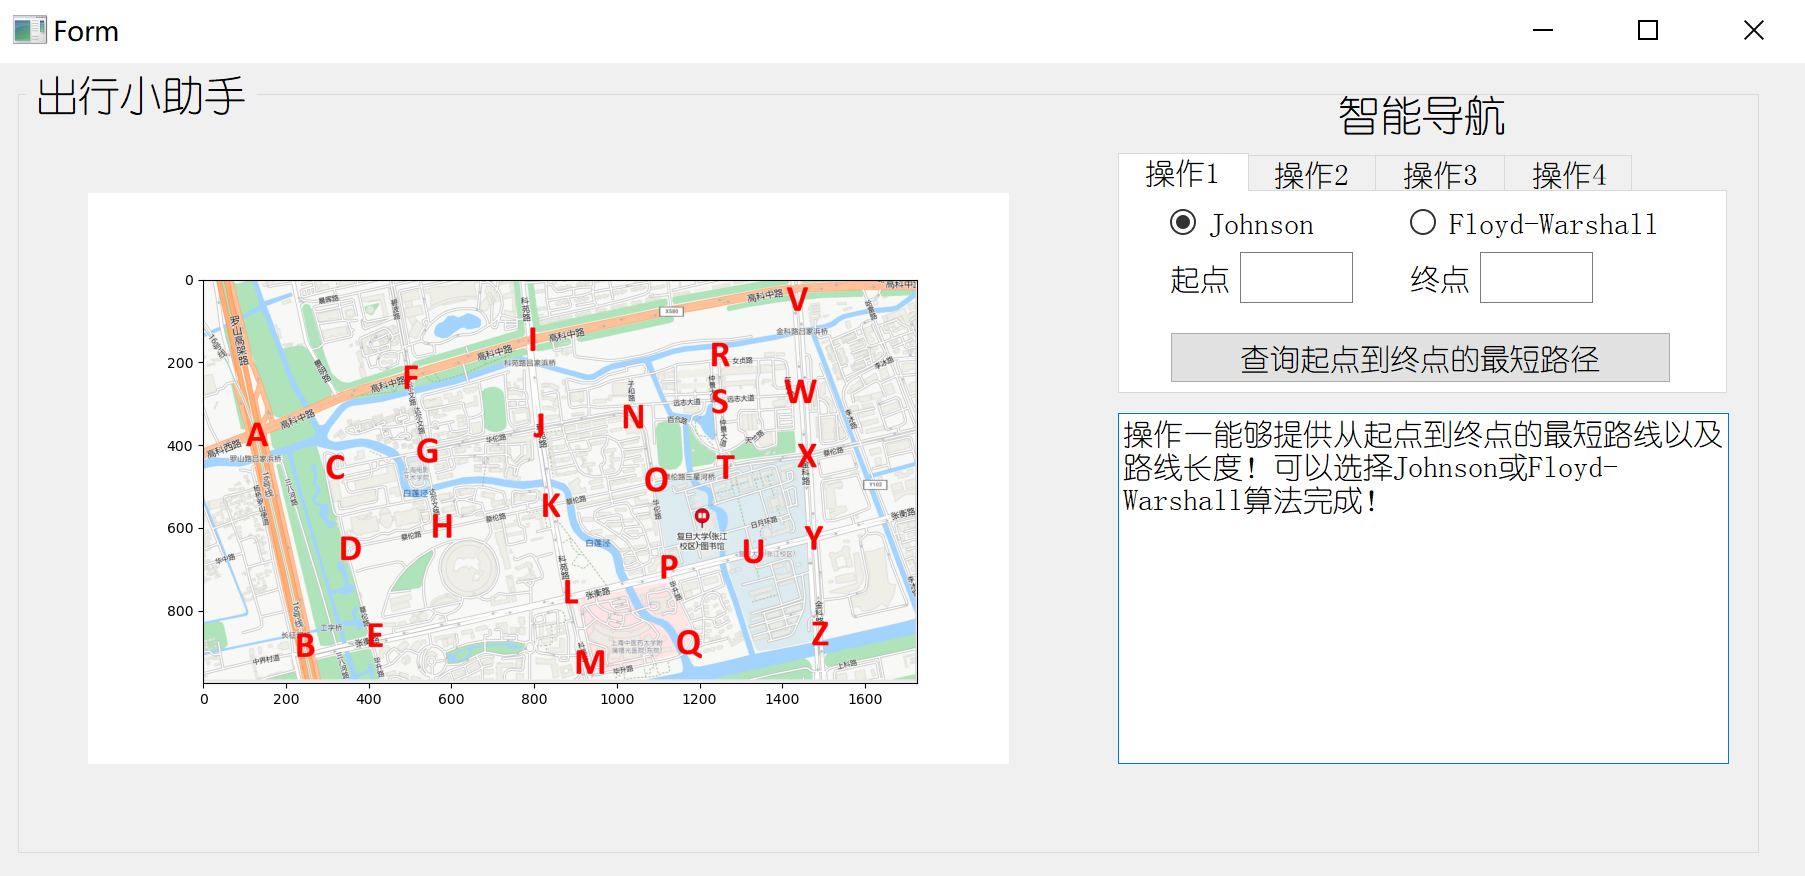
\includegraphics[width=0.5\textwidth]{image//启动界面.png}} 
% 	\caption{启动界面} 
% \end{figure}


\subsection{操作一}
操作一的初始界面如图\ref{op1.init}所示,默认选择Johnson's algorithm,右下角的展示框中会
简要介绍该操作的功能。
\begin{figure}[H]
	\centering
	{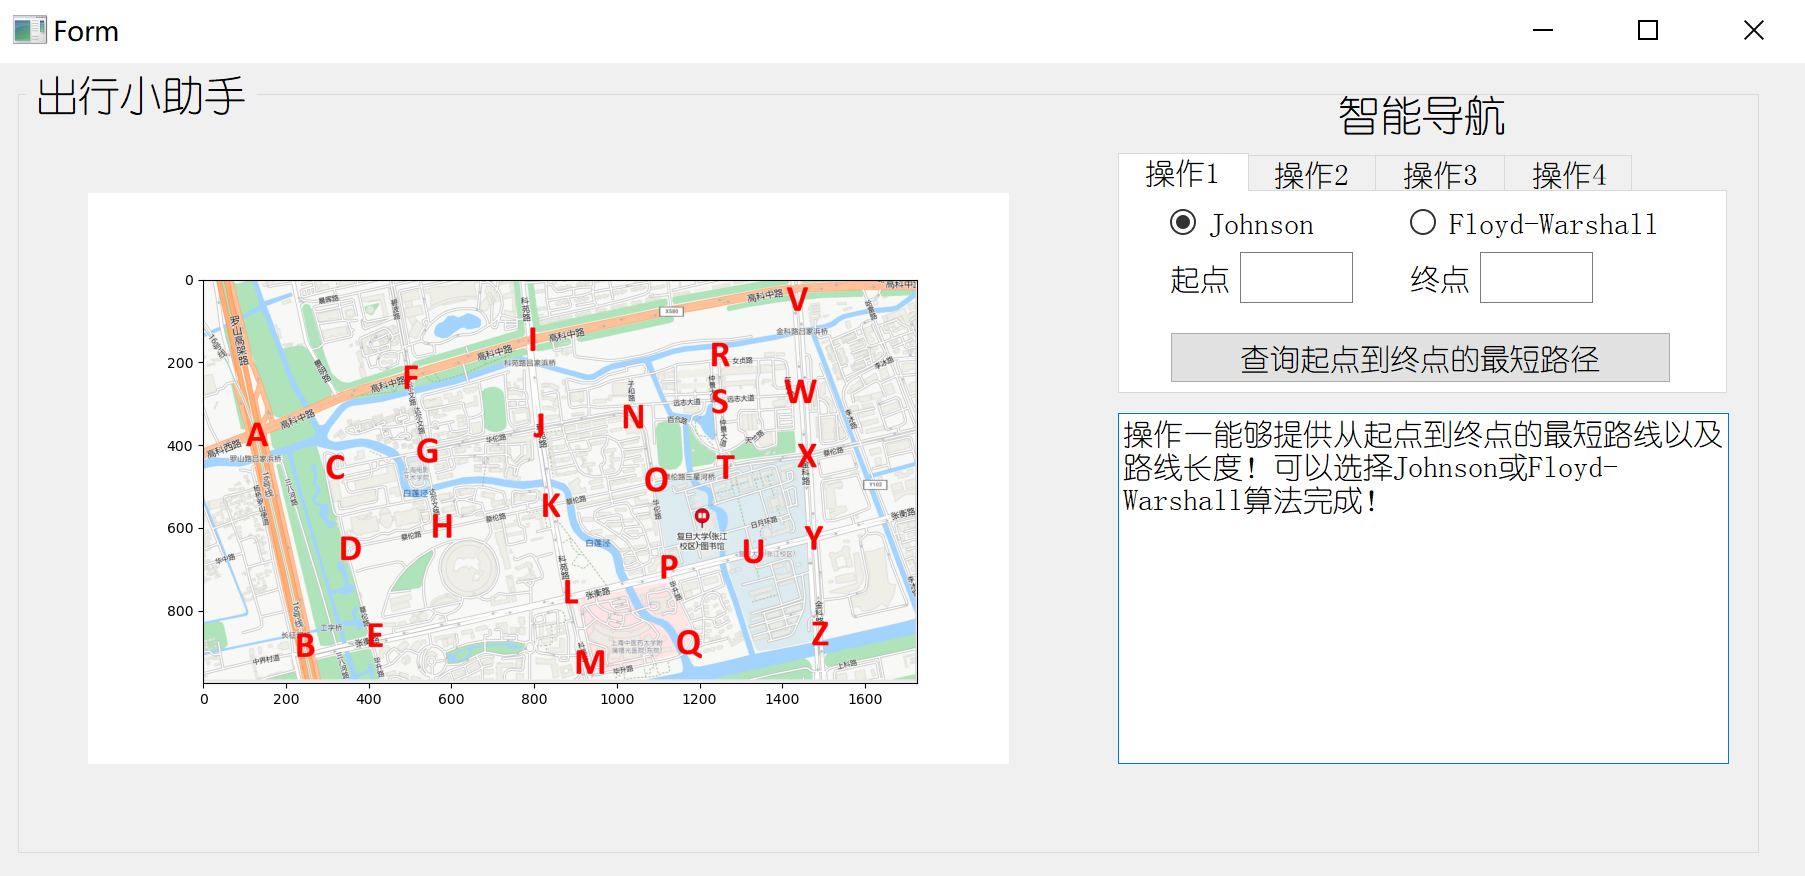
\includegraphics[width=0.75\textwidth]{image//启动界面.png}} 
	\caption{操作一初始界面} \label{op1.init}
\end{figure}

在地图上任意点击,系统会计算距离鼠标点击点的位置最近的字母作为用户所选的点。
在地图上点击两个点,作为起点和终点,系统会帮助用户在输入框中填入起点和终点的字母,
然后点击“查询起点到终点的最短路径”按钮,效果如图\ref{op1.result}所示。
左侧的地图上会用黄色绘制出最短路径,右侧的展示框中会展示最短路径经过的节点以及顺序,
以及最短路径长度。
\begin{figure}[H]
	\centering
	{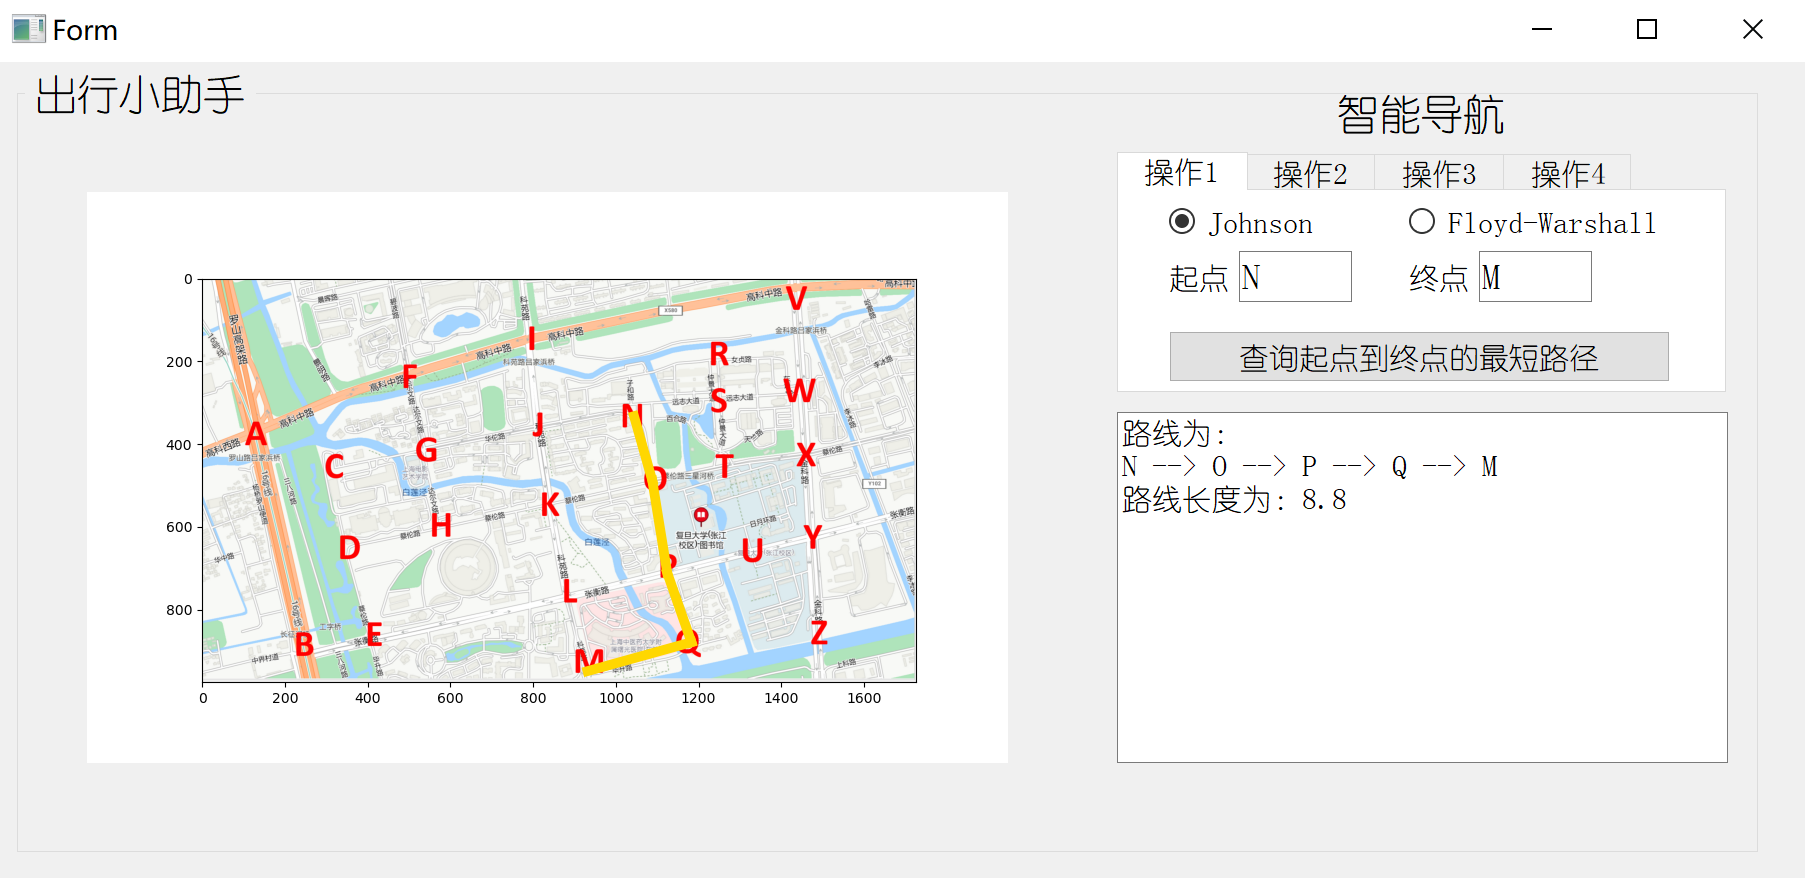
\includegraphics[width=0.75\textwidth]{image//操作一结果.png}} 
	\caption{操作一的查询效果} \label{op1.result}
\end{figure}
如果需要查询另外两点之间的最短路径,只需要再次在地图上任意点击两个点,
作为新的起点和新的终点,
然后点击查询,系统便会擦除原本的路径,绘制新的路径。

GUI也支持用户自行在输入框中输入字母作为起点和终点。但是,如果用户输入的字符
不在地图中,则视为非法输入,系统启动防错机制,要求用户输入正确的起点和终点,
如图\ref{op1.error}所示。
\begin{figure}[H]
	\centering
	{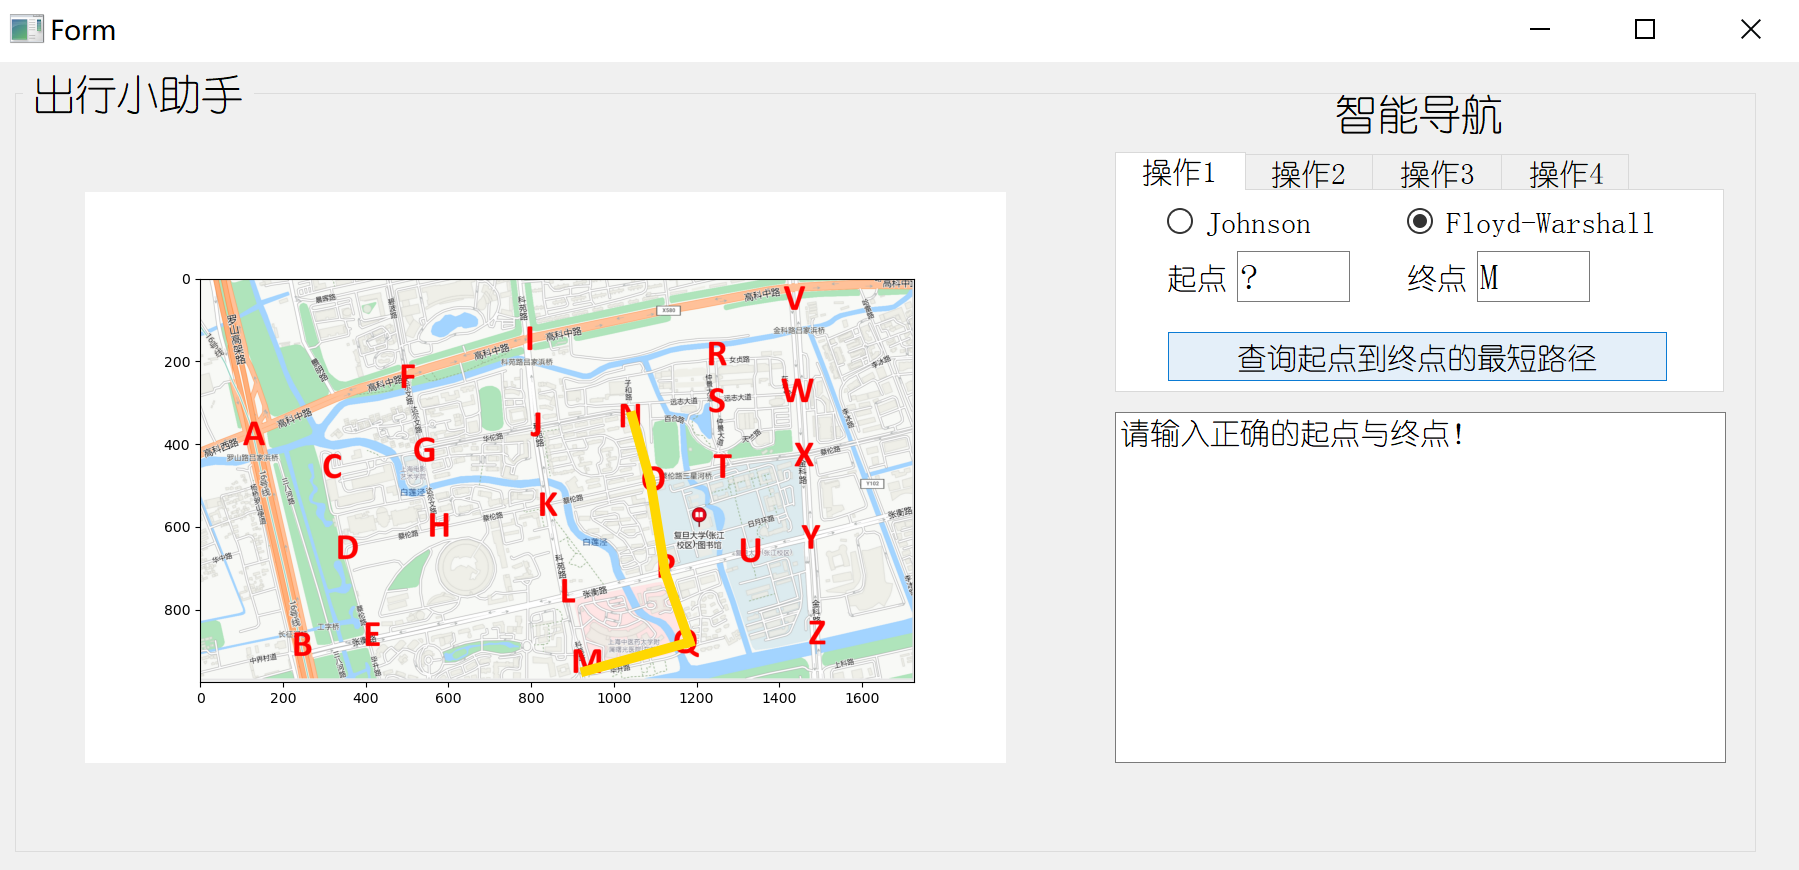
\includegraphics[width=0.75\textwidth]{image//操作一纠错.png}} 
	\caption{操作一的防错机制} \label{op1.error}
\end{figure}

\subsection{操作二}
操作二的初始界面如图\ref{op2.init}所示,默认选择Johnson's algorithm,右下角的展示框中会
简要介绍该操作的功能。
\begin{figure}[H]
	\centering
	{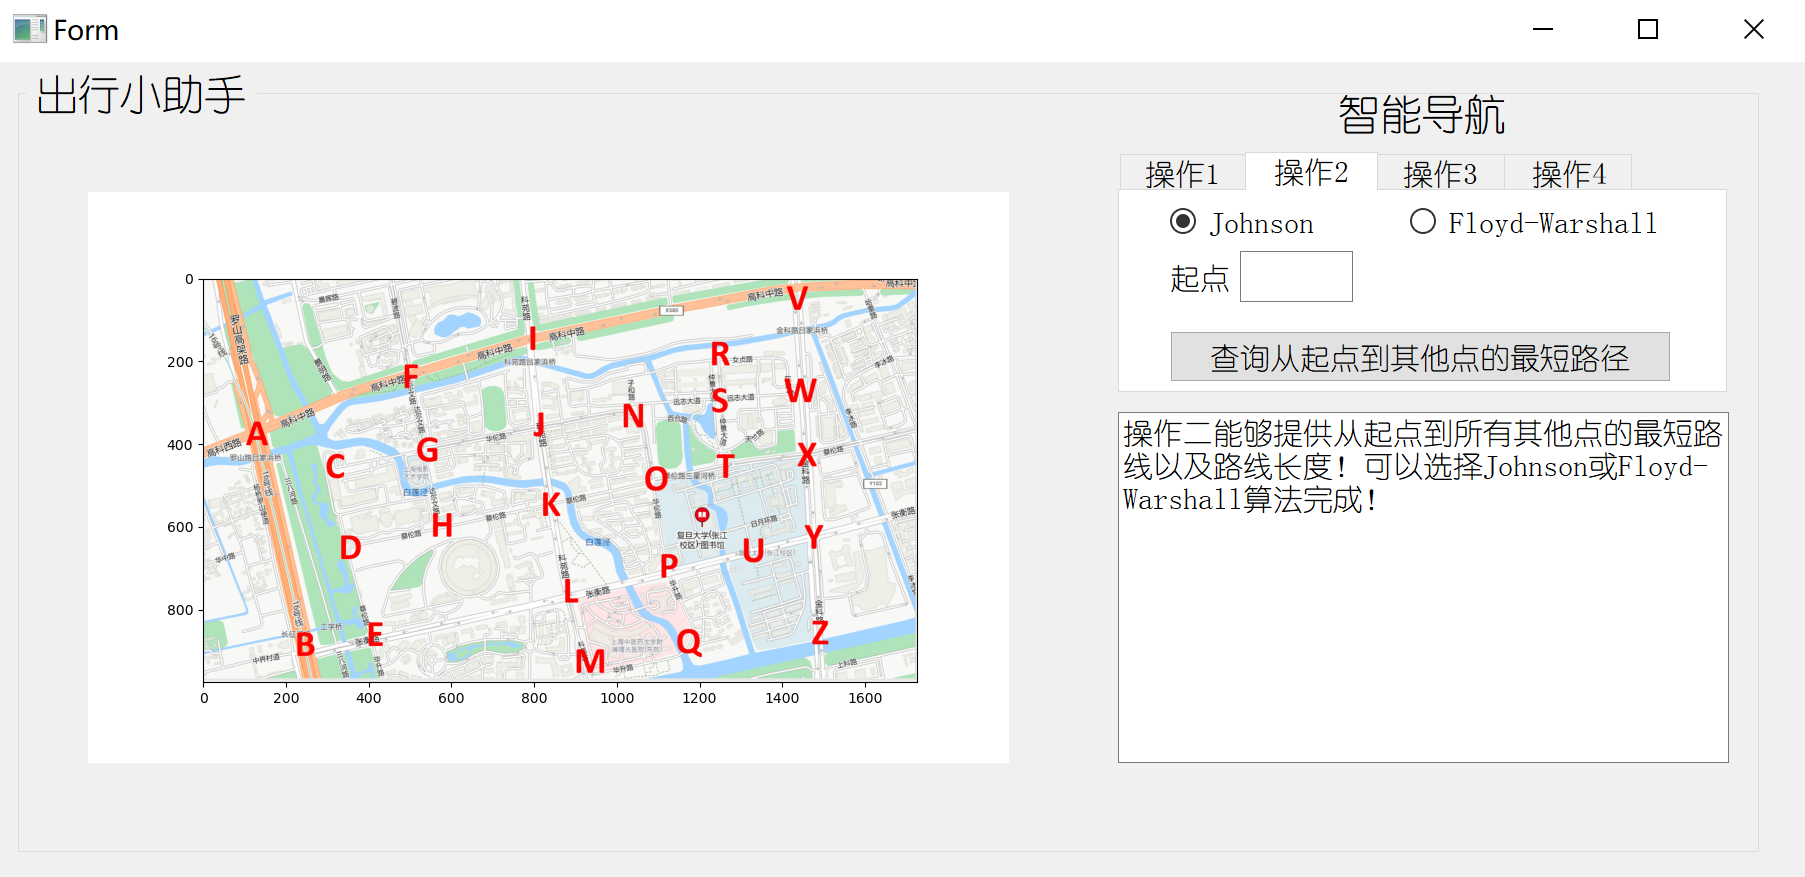
\includegraphics[width=0.75\textwidth]{image//操作二初始界面.png}} 
	\caption{操作二的初始界面} \label{op2.init}
\end{figure}

在地图上任意点击,系统会计算距离鼠标点击点的位置最近的字母作为用户所选的起点。
点击“查询从起点到其他点的最短路径”,效果如图\ref{op2.result}所示。右下角的展示框中会输出
从起点到所有其他终点的最短路径经过的节点与顺序,以及相应的路径长度。
\begin{figure}[H]
	\centering
	{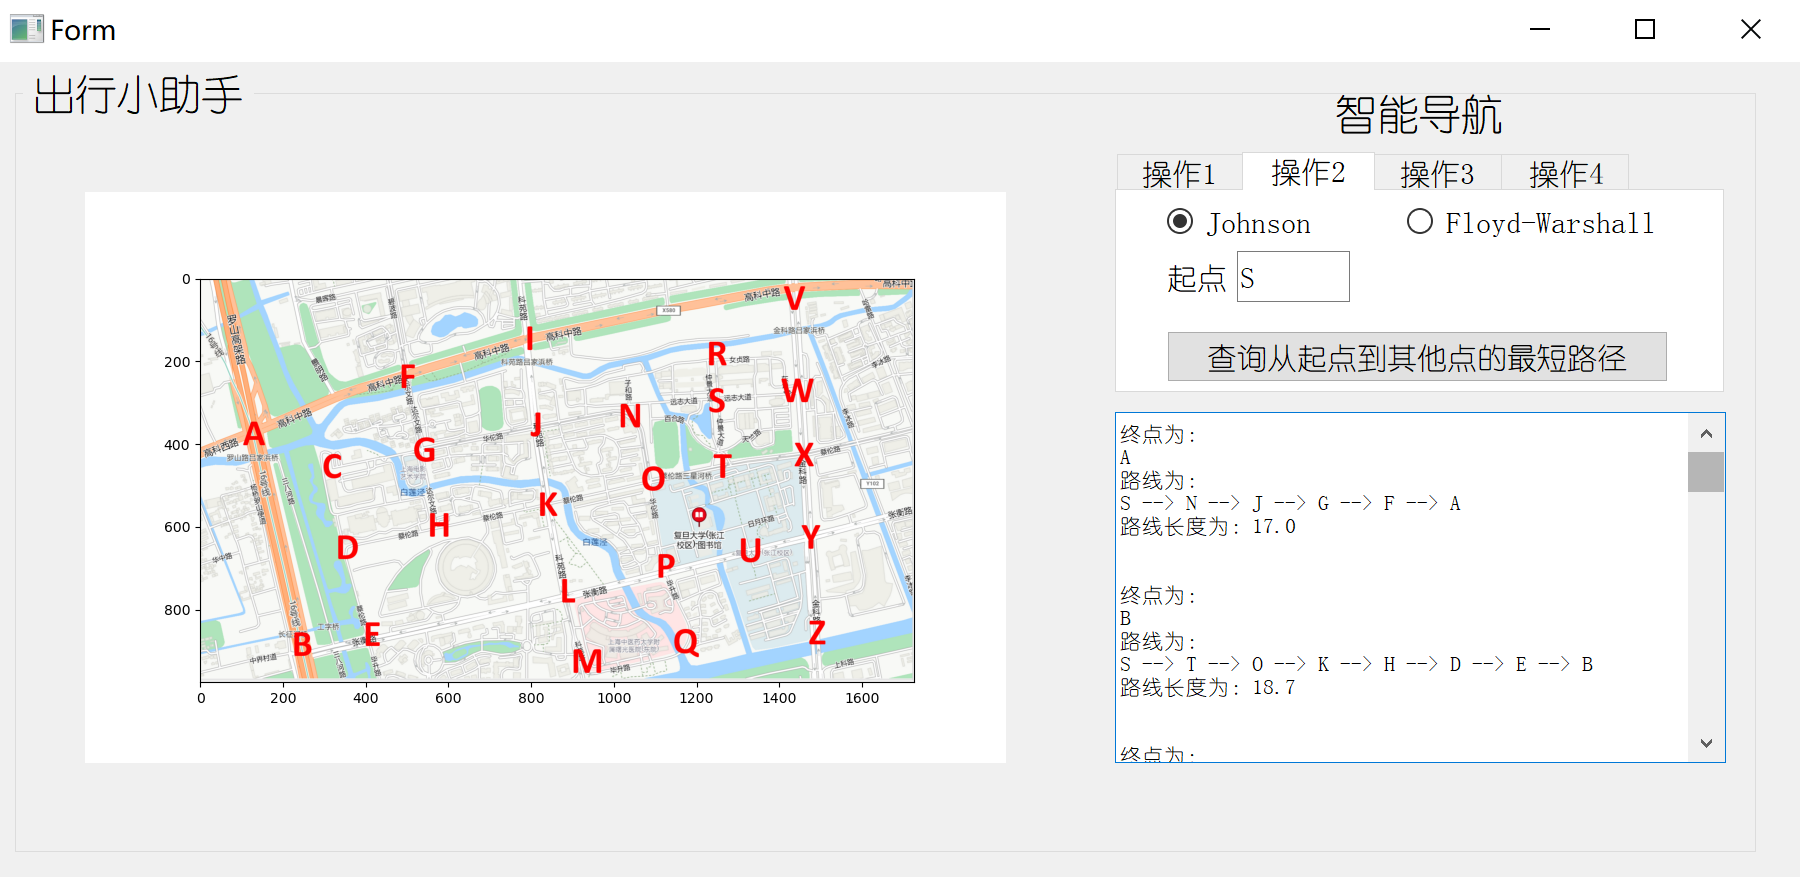
\includegraphics[width=0.75\textwidth]{image//操作二结果.png}} 
	\caption{操作二的查询效果} \label{op2.result}
\end{figure}

此外,操作二也支持用户在输入框中手动输入起点名称,并且也有与操作一类似的防错机制,
此处不再赘述。

\subsection{操作三}
操作三的初始界面如图\ref{op3.init}所示,默认选择Krustal's algorithm。 但该算法只能找到第一棵最小生成树。
如果需要找到第二棵最小生成树,就需要选择Prim's algorithm。
\begin{figure}[H]
	\centering
	{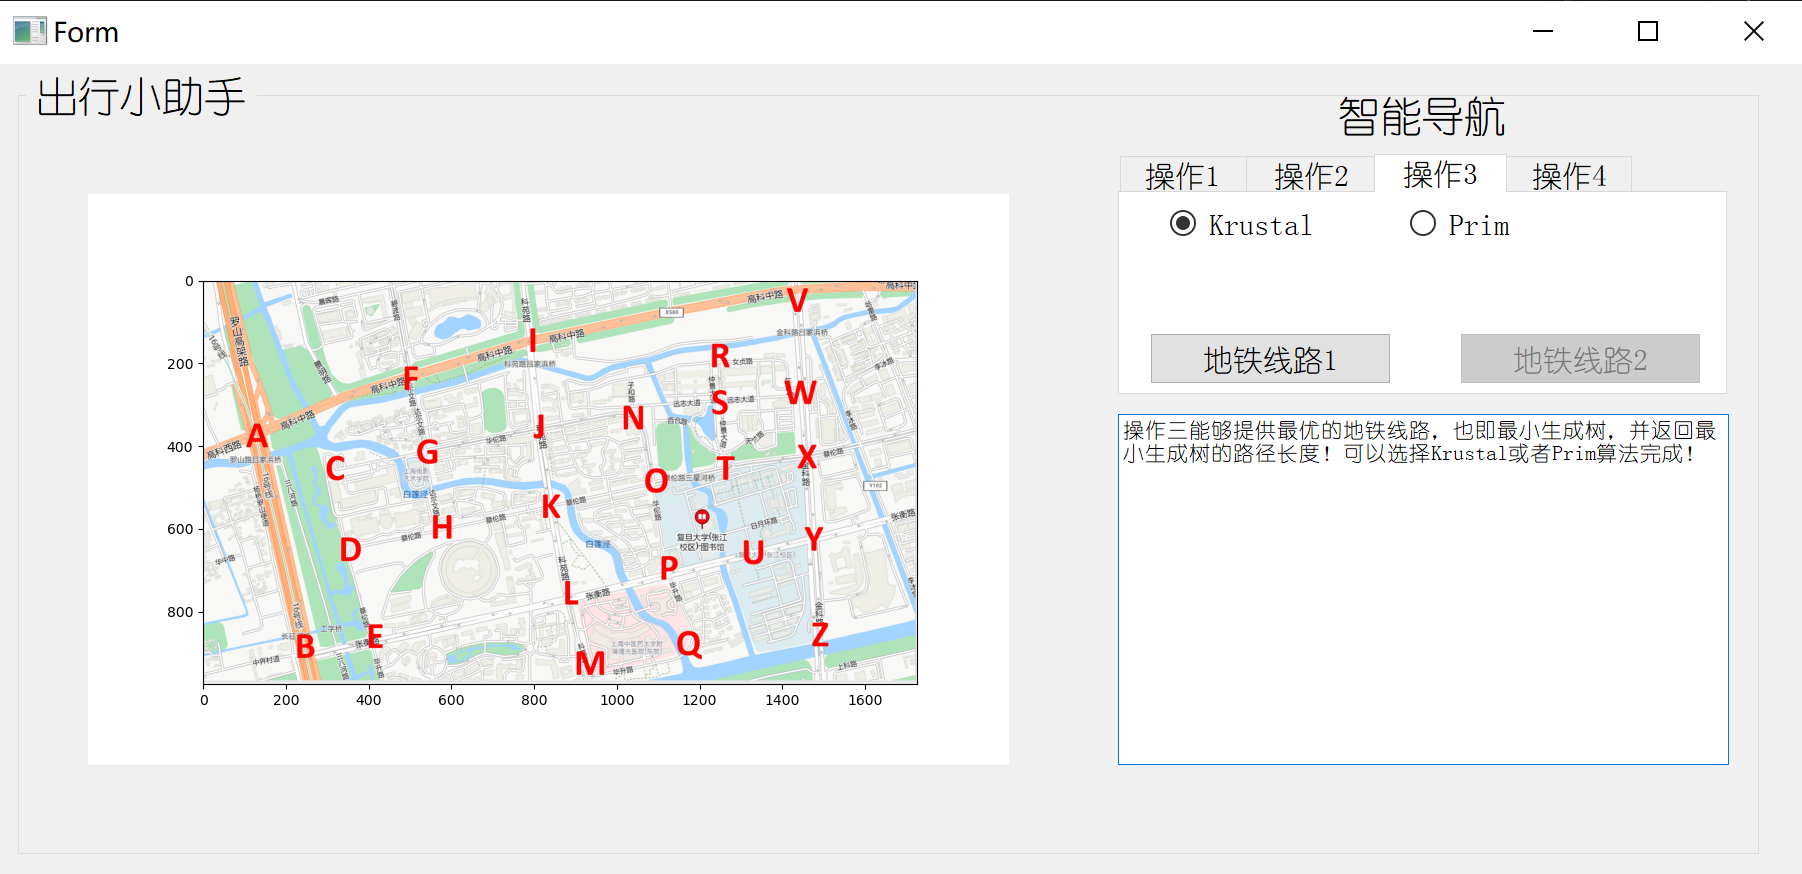
\includegraphics[width=0.75\textwidth]{image//操作三初始界面.png}} 
	\caption{操作三的初始界面} \label{op3.init}
\end{figure}

在选择Prim's algorithm的情况下,分别点击“地铁路线1”和“地铁路线2”,系统会分别在图中用黄色
绘制出最小生成树所包含的边长,并且在右下角的展示框中输出最小生成树的总长度,
以及包含的edge。效果分别如图\ref{op3.result.1}和图\ref{op3.result.2}所示。
\begin{figure}[H]
    \centering
    \subfigure[第一条地铁线路查询结果]
    {\label{op3.result.1} 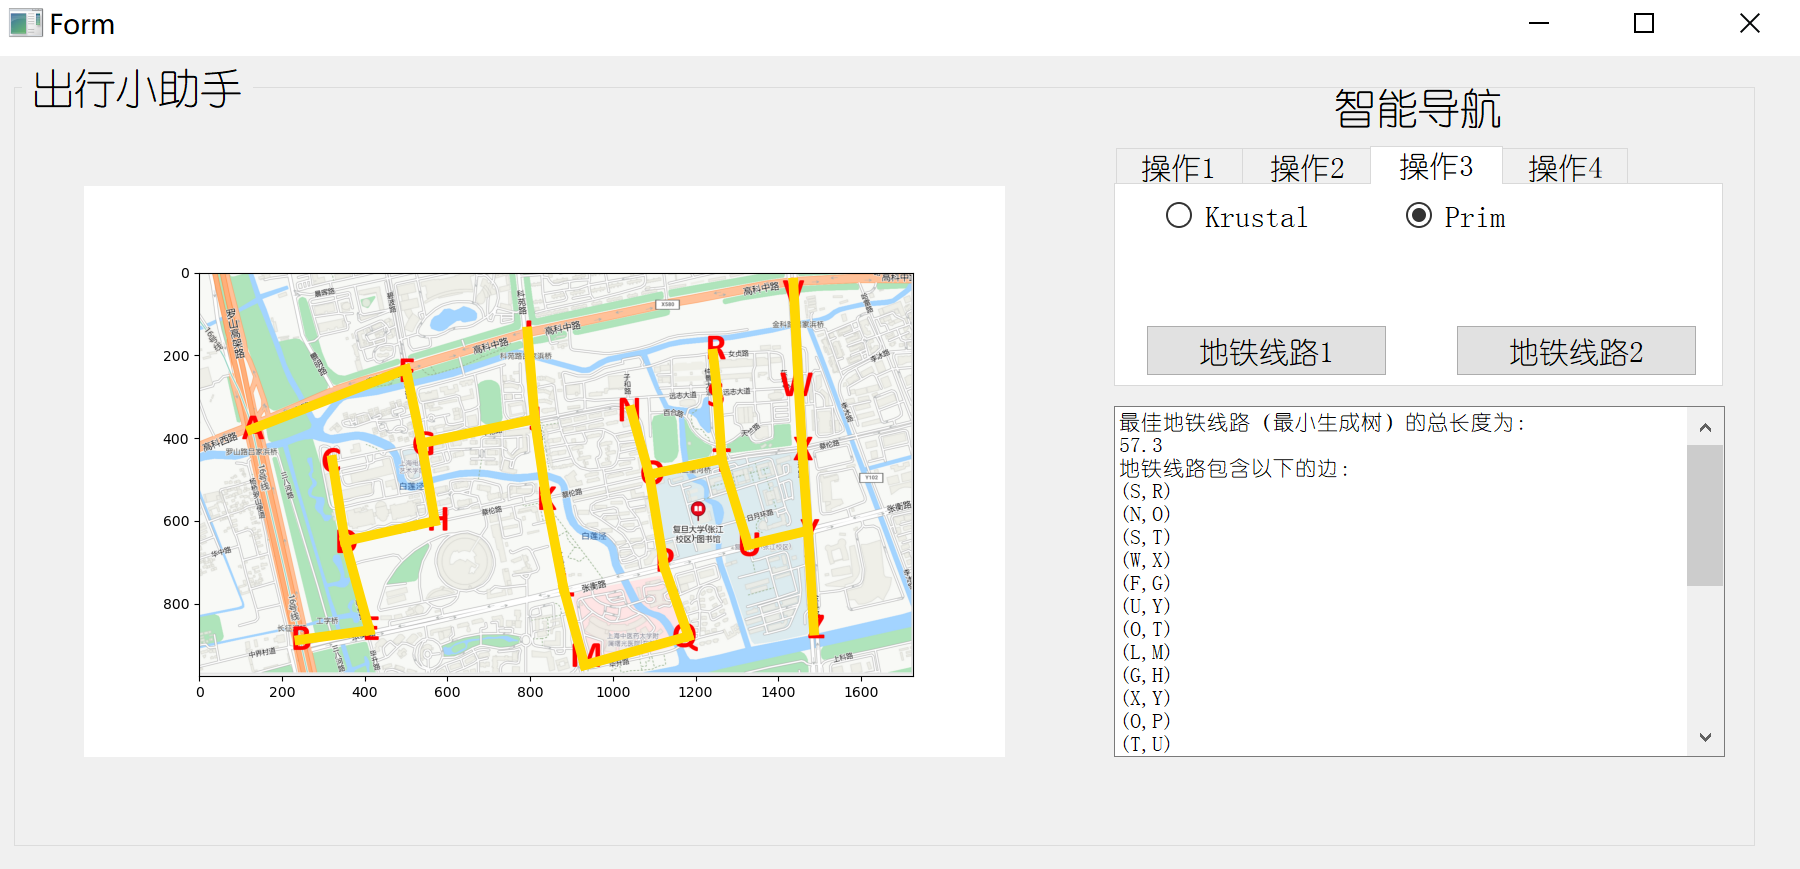
\includegraphics[width=0.45\textwidth]{image//操作三线路一.png}}
    \,    
    \subfigure[第二条地铁线路查询结果]
    {\label{op3.result.2} 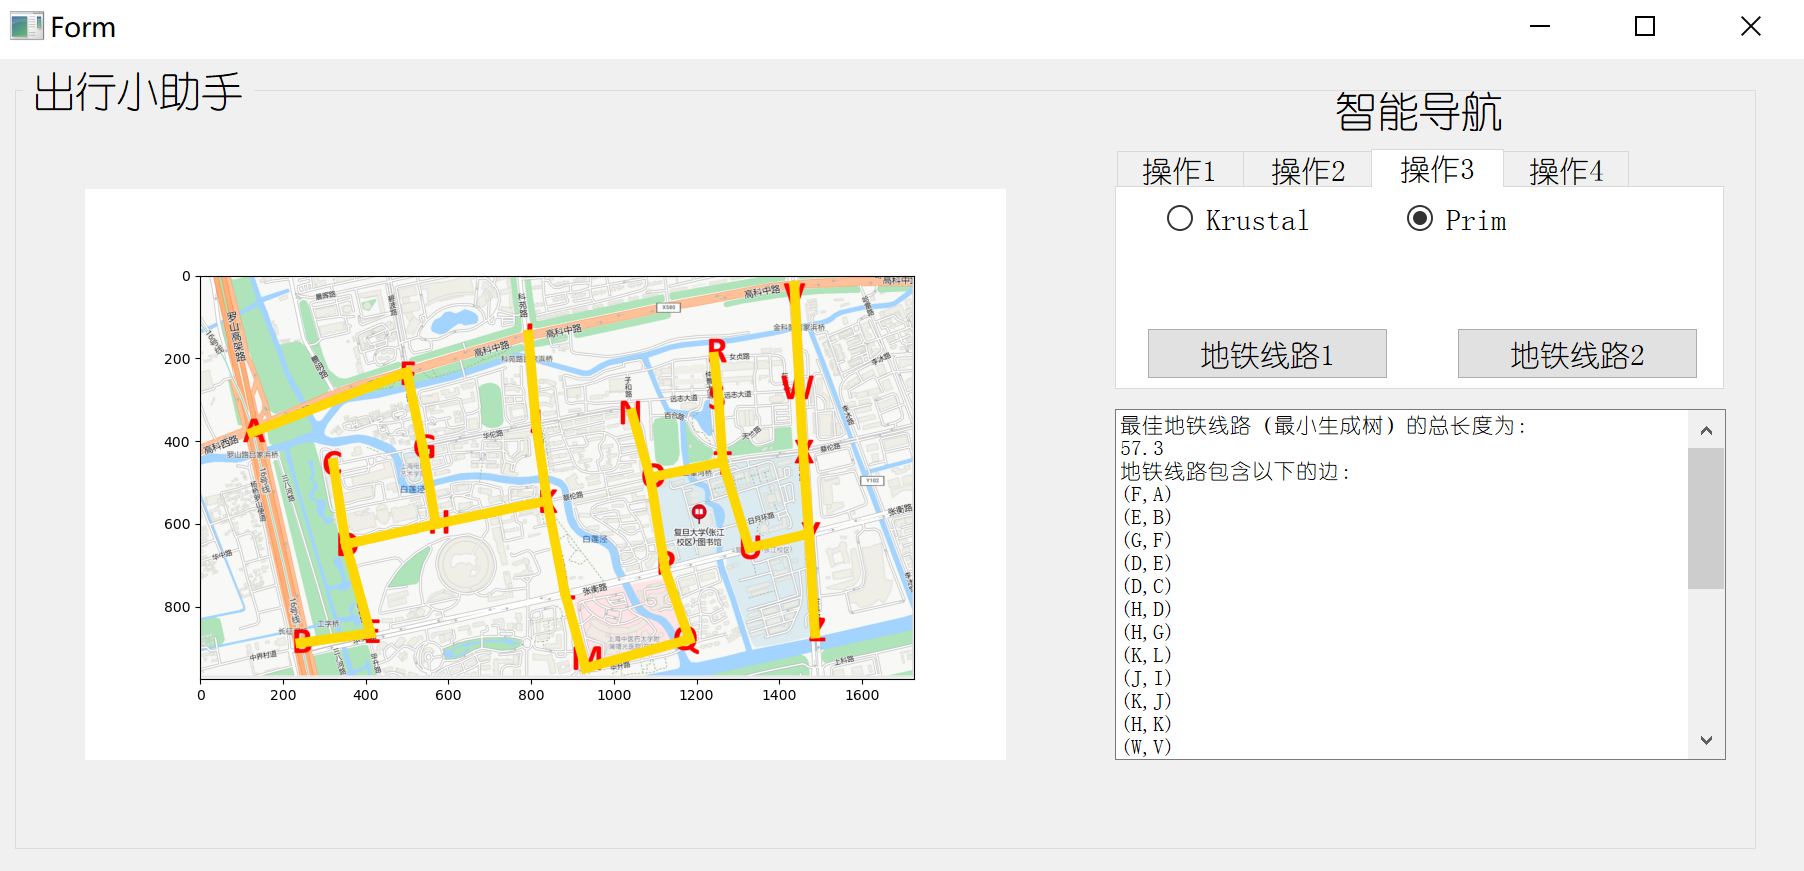
\includegraphics[width=0.45\textwidth]{image//操作三路线二.png}}
    \caption{操作三的查询效果} \label{op3.result}
\end{figure}

\subsection{操作四}
操作四的初始界面如图\ref{op4.init}所示。
\begin{figure}[H]
	\centering
	{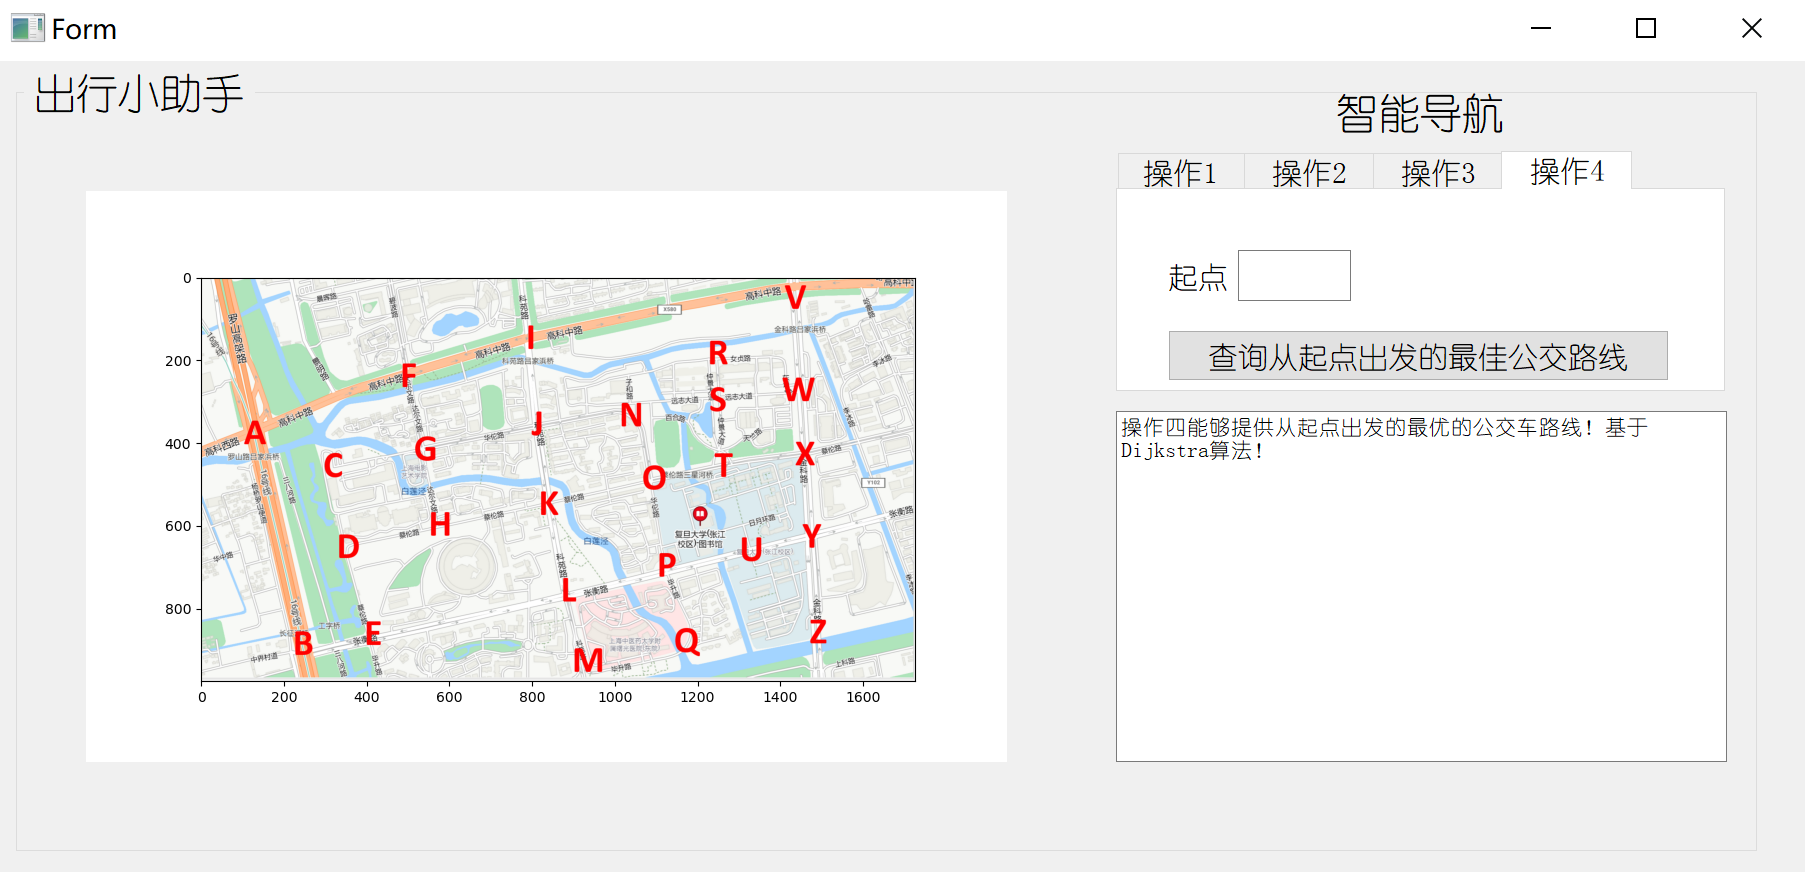
\includegraphics[width=0.75\textwidth]{image//操作四初始界面.png}} 
	\caption{操作四的初始界面} \label{op4.init} 
\end{figure}

在地图上任意点击,系统会计算距离鼠标点击点的位置最近的字母作为用户所选的起点。
点击“查询从起点出发的最佳公交路线”,效果如图\ref{op4.result}所示。右下角的展示框中会输出
以用户选定字母为起点的最佳公交路线的总长度,以及包含的edge,效果如图\ref{op4.result}所示。
\begin{figure}[H]
	\centering
	{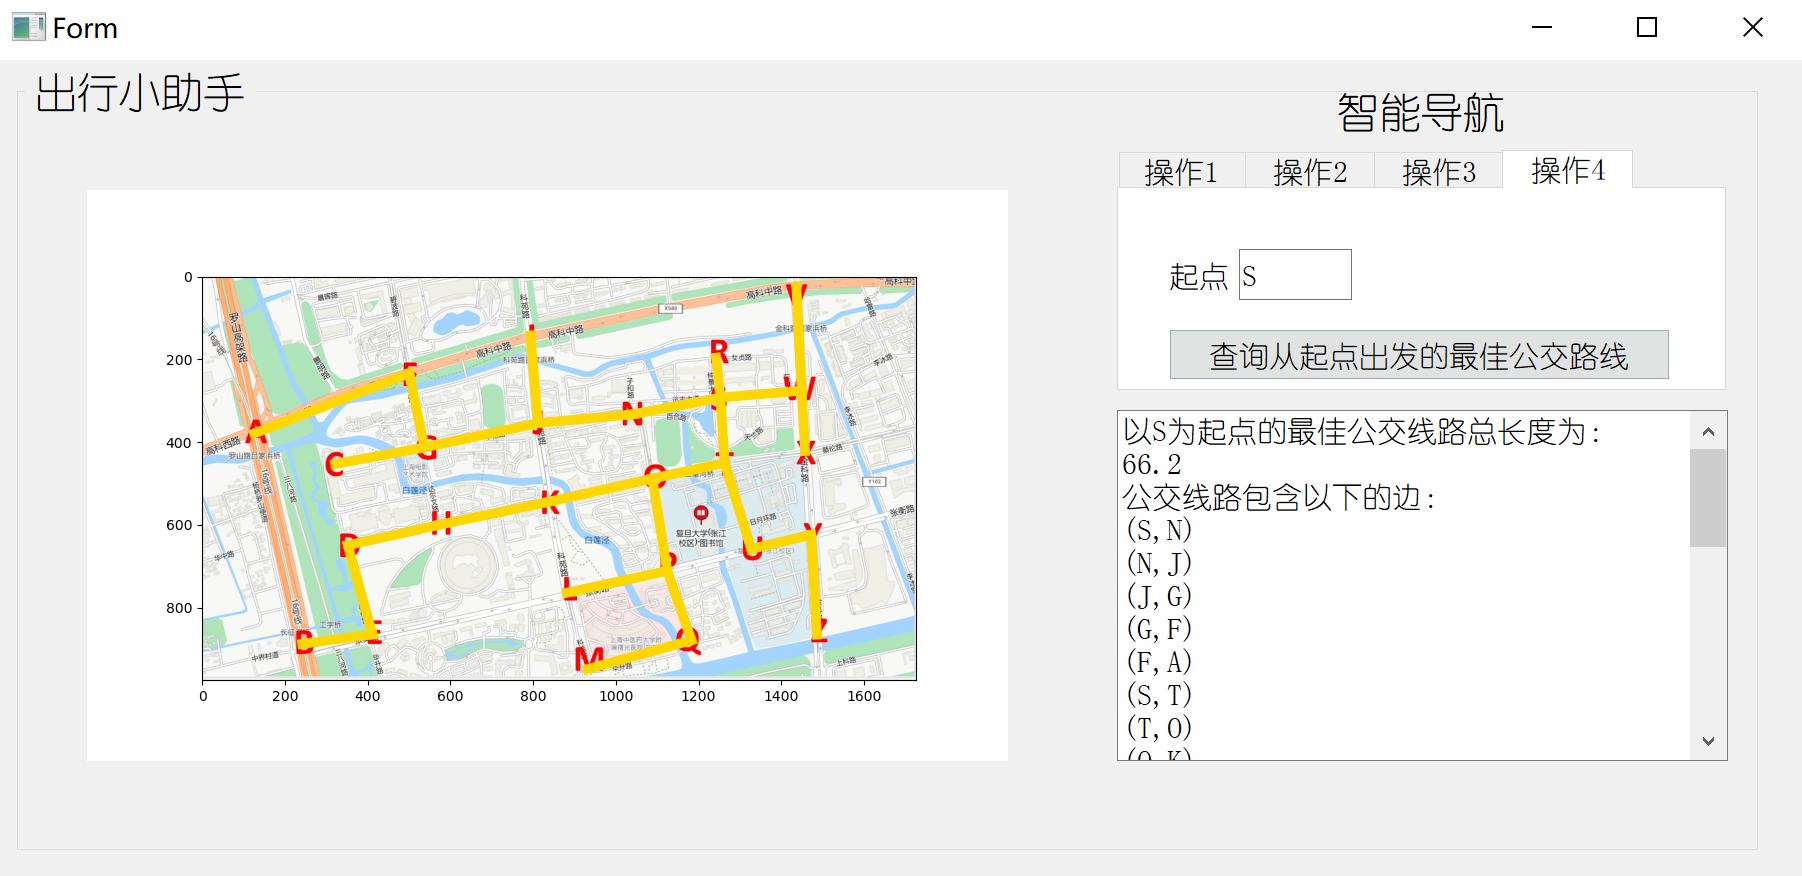
\includegraphics[width=0.75\textwidth]{image//操作四结果.png}} 
	\caption{操作四的查询效果} \label{op4.result} 
\end{figure}

此外,操作四也支持用户在输入框中手动输入起点名称,并且也有与操作一类似的防错机制,
此处不再赘述。

\section{算法复杂度分析}
\subsection{操作一和操作二的算法复杂度分析}
操作一和操作二是基于Floyd-Warshall算法和Johnson算法实现最短路径查找的。
请注意,只有在\textbf{第一次运行}Floyd-Warshall算法和Johnson算法时,才会计算各点之间的最短路径。
再次调用时,不再重复计算,只会输出结果,输出结果的复杂度为$\mathcal{O}(E)$。

以下是对第一次调用操作一或操作二时,执行Floyd-Warshall算法和Johnson算法的复杂度分析。

\subsubsection{Floyd-Warshall算法复杂度分析}
算法需要维护两个矩阵$D$和$\Pi$,空间复杂度为$\mathcal{O}(V^2)$。矩阵$D$的更新过程为:
\begin{equation}
	d_{ij}^{(k)} = 
	\begin{cases}
		w_{i,j} & \text{if  $k=0$} \\
		\min (d_{ij}^{(k-1)}, d_{ik}^{(k-1)} + d_{kj}^{(k-1)}) & \text{if  $k\ge 1$}
	\end{cases} \end{equation}
		


矩阵$\Pi$的更新过程为:
\begin{equation}
	\pi_{ij}^{(k)} = 
	\begin{cases}
		\pi_{ij}^{(k-1)} & \text{if  $d_{ij}^{(k-1)}\le d_{ik}^{(k-1)} + d_{kj}^{(k-1)}$} \\
		\pi_{kj}^{(k-1)} & \text{if  $d_{ij}^{(k-1)} > d_{ik}^{(k-1)} + d_{kj}^{(k-1)}$} 
	\end{cases} \end{equation}

对矩阵$D$和$Pi$需要做$V$轮次更新,每次更新的时间复杂度为$\mathcal{O}(V^2)$,
因此Floyd-Warshall算法的时间复杂度为$\mathcal{O}(V^3)$。

\subsubsection{Johnson算法复杂度分析}
Johnson算法先使用带有一个辅助节点的增广图,通过运行Bellman-Ford算法来检查是否
存在负环。Bellman-Ford算法运行$V$轮,前$V-1$轮用于寻找从辅助节点出发的最短路径,
最后一轮用于检查是否存在负环。每一轮需要对$E$条edge进行更新。因此,
Bellman-Ford算法的时间复杂度为$\mathcal{VE}$。

在没有负环的情况下,对每一条边进行权重重置,该步骤的复杂度为$\mathcal{O}(V+E)$。
然后对每一个点执行Dijkstra算法,每一次运行Dijkstra算法的复杂度是$\mathcal{O}(E\lg V)$,
对$V$个节点,需要运行$V$轮,则复杂度为$\mathcal{O}(VE\lg V)$。

综上,Johnson算法的复杂度为$\mathcal{O}(VE\lg V)$。

\subsection{操作三的算法复杂度分析}
操作三提供了两种寻找最小生成树(MST)的方法,分别是Krustal算法和Prim算法。以下
是对这两种算法的复杂度分析。
\subsubsection{Krustal算法复杂度分析}
Krustal算法首先要对$V$个节点各自建立并查集。
然年对所有的边长进行排序,如果采用基于比较的排序,则复杂度为$\mathcal{O}(E\lg E)$。

然后遍历每一条edge,根据edge的两个端点是否在同一个集合内判断是否向最小生成树
中加入这条edge。判断edge是否加入MST的时候,需要对并查集进行查询
和并集两种操作。在实现并查集的时候,我使用了union by rank和path compression两个技巧,
使得对并查集进行$\mathcal{O}(V+E)$次操作的复杂度能够下降到$\mathcal{O}((V+E)\,\alpha(V))$,其中
$\alpha(V)$在本题中可以近似为常数。
本题中$E>V$,因此有$\mathcal{O}((V+E)\,\alpha(V)) = \mathcal{O}(E\,\alpha(V)) = \mathcal{O}(E)$,
因此判断edge是否加入MST的过程复杂度近似为$\mathcal{O}(E)$。

综上,基于并查集实现的Krustal算法复杂度为$\mathcal{O}(E\lg E)$。考虑到本题中有$E<V^2$,
则$\lg E = \mathcal{O}(\lg V)$,
因此也可以认为$\mathcal{O}(E\lg E) = \mathcal{O}(E\lg V)$。

\subsubsection{Prim算法复杂度分析}
Prim算法是基于\textbf{最小堆}实现的。建立最小堆的复杂度为$\mathcal{O}(V)$。
算法需要对$V$个节点进行遍历,每次从最小堆中取出权重最小的节点,该操作复杂度为$\mathcal{O}(\lg V)$,
由于要从最小堆中进行$V$次取出最小节点的操作,则该部分复杂度为$\mathcal{O}(V\lg V)$。

在遍历的过程中,需要对每个节点的所有邻接节点进行decrease-key操作,
decrease-key操作的复杂度也为$\mathcal{O}(\lg V)$。
注意到邻接表的空间复杂度为$\mathcal{O}(E)$,因此所有decrease-key操作的复杂度为$\mathcal{O}(E\lg V)$。

由于$E>V$,则Prim算法的复杂度为$\mathcal{O}(V + V\lg V + E\lg V) = \mathcal{O}(E\lg V) $,
与Krustal算法复杂度接近。

\subsection{操作四算法复杂度分析}
操作四基于对Dijkstra算法的改编实现。使用的数据结构为\textbf{最小堆}。
算法过程与Prim算法高度相似,故此处仅做简要描述。
类似于Prim算法,同样需要对$V$个节点进行遍历,每次从最小堆中取出权重最小的节点。
在遍历的过程中,需要对每个节点的所有邻接节点进行decrease-key操作,一共做$\mathcal{O}(E)$次的decrease-key操作。
因此,Dijkstra算法的复杂同样也为$\mathcal{O}(E\lg V)$。

注意到操作四还需要把从起点到图中其他点的最短路径所包含边取并集作为最佳公交路线返回,
对各最短路径取并集的复杂度为$\mathcal{O}(VE)$。因此,尽管Dijkstra算法的复杂度是$\mathcal{O}(E\lg V)$,
但是要实现操作四的功能,复杂度则是$\mathcal{O}(E\lg V + VE) = \mathcal{O}(VE)$。

\section{Bonus得分点汇总}
\begin{enumerate}

	\item 为用户提供Johnson's algorithm和Floyd-Warshall algorithm\textbf{两种}全局最短路径算法以实现操作一和操作二,
		实现Johnson's algorithm时还完成了的单源最短路径算法Bellman-Frod算法;
	\item 为用户提供Krustal's algorithm和Prim's algorithm\textbf{两种}最小生成树算法以实现操作三,实现Krustal算法时候
		还完成了Disjoint数据结构的实现;
	\item 为用户提供\textbf{地图自由选点}功能,也允许用户在输入框中\textbf{手动}输入起点和终点名称,且具备防错机制。
	
\end{enumerate}

\end{document}

% \begin{figure}[H]
% 	\centering
% 	{\includegraphics[width=0.35\textwidth]{image//ignorance.png}} 
% 	\caption{} \label{} 
% \end{figure}


% \lstinputlisting[style = Python,
% caption={Python codes},
% label = {efficient},
% linerange={110-125}]{exercise3.py} 


% \begin{figure}[H]
%     \centering
%     \subfigure[patch size = 11]
%     {\label{} \includegraphics[width=0.49\textwidth]{image//local equalization with patch size = 11.jpg}}
%     \,    
%     \subfigure[patch size = 51]
%     {\label{} \includegraphics[width=0.49\textwidth]{image//local equalization with patch size = 51.jpg}}
%     \,
%     \subfigure[patch size = 151]
%     {\label{} \includegraphics[width=0.49\textwidth]{image//local equalization with patch size = 151.jpg}}
%     \,    
%     \subfigure[patch size = 201]
%     {\label{} \includegraphics[width=0.49\textwidth]{image//local equalization with patch size = 201.jpg}}
%     \caption{local equalization with different patch sizes}\label{} 
% \end{figure}
